% Options for packages loaded elsewhere
\PassOptionsToPackage{unicode}{hyperref}
\PassOptionsToPackage{hyphens}{url}
%
\documentclass[
  10pt,
  ignorenonframetext,
]{beamer}
\title{Présentation du machine learning}
\author{Mohamed Essaied Hamrita}
\date{IHEC - Sousse}

\usepackage{pgfpages}
\setbeamertemplate{caption}[numbered]
\setbeamertemplate{caption label separator}{: }
\setbeamercolor{caption name}{fg=normal text.fg}
\beamertemplatenavigationsymbolsempty
% Prevent slide breaks in the middle of a paragraph
\widowpenalties 1 10000
\raggedbottom
\setbeamertemplate{part page}{
  \centering
  \begin{beamercolorbox}[sep=16pt,center]{part title}
    \usebeamerfont{part title}\insertpart\par
  \end{beamercolorbox}
}
\setbeamertemplate{section page}{
  \centering
  \begin{beamercolorbox}[sep=12pt,center]{part title}
    \usebeamerfont{section title}\insertsection\par
  \end{beamercolorbox}
}
\setbeamertemplate{subsection page}{
  \centering
  \begin{beamercolorbox}[sep=8pt,center]{part title}
    \usebeamerfont{subsection title}\insertsubsection\par
  \end{beamercolorbox}
}
\AtBeginPart{
  \frame{\partpage}
}
\AtBeginSection{
  \ifbibliography
  \else
    \frame{\sectionpage}
  \fi
}
\AtBeginSubsection{
  \frame{\subsectionpage}
}
\usepackage{amsmath,amssymb}
\usepackage{lmodern}
\usepackage{iftex}
\ifPDFTeX
  \usepackage[T1]{fontenc}
  \usepackage[utf8]{inputenc}
  \usepackage{textcomp} % provide euro and other symbols
\else % if luatex or xetex
  \usepackage{unicode-math}
  \defaultfontfeatures{Scale=MatchLowercase}
  \defaultfontfeatures[\rmfamily]{Ligatures=TeX,Scale=1}
\fi
\usefonttheme{structurebold}
% Use upquote if available, for straight quotes in verbatim environments
\IfFileExists{upquote.sty}{\usepackage{upquote}}{}
\IfFileExists{microtype.sty}{% use microtype if available
  \usepackage[]{microtype}
  \UseMicrotypeSet[protrusion]{basicmath} % disable protrusion for tt fonts
}{}
\makeatletter
\@ifundefined{KOMAClassName}{% if non-KOMA class
  \IfFileExists{parskip.sty}{%
    \usepackage{parskip}
  }{% else
    \setlength{\parindent}{0pt}
    \setlength{\parskip}{6pt plus 2pt minus 1pt}}
}{% if KOMA class
  \KOMAoptions{parskip=half}}
\makeatother
\usepackage{xcolor}
\IfFileExists{xurl.sty}{\usepackage{xurl}}{} % add URL line breaks if available
\IfFileExists{bookmark.sty}{\usepackage{bookmark}}{\usepackage{hyperref}}
\hypersetup{
  pdftitle={Présentation du machine learning},
  pdfauthor={Mohamed Essaied Hamrita},
  hidelinks,
  pdfcreator={LaTeX via pandoc}}
\urlstyle{same} % disable monospaced font for URLs
\newif\ifbibliography
\usepackage{graphicx}
\makeatletter
\def\maxwidth{\ifdim\Gin@nat@width>\linewidth\linewidth\else\Gin@nat@width\fi}
\def\maxheight{\ifdim\Gin@nat@height>\textheight\textheight\else\Gin@nat@height\fi}
\makeatother
% Scale images if necessary, so that they will not overflow the page
% margins by default, and it is still possible to overwrite the defaults
% using explicit options in \includegraphics[width, height, ...]{}
\setkeys{Gin}{width=\maxwidth,height=\maxheight,keepaspectratio}
% Set default figure placement to htbp
\makeatletter
\def\fps@figure{htbp}
\makeatother
\setlength{\emergencystretch}{3em} % prevent overfull lines
\providecommand{\tightlist}{%
  \setlength{\itemsep}{0pt}\setlength{\parskip}{0pt}}
\setcounter{secnumdepth}{-\maxdimen} % remove section numbering
\ifLuaTeX
  \usepackage{selnolig}  % disable illegal ligatures
\fi

\begin{document}
\frame{\titlepage}

\begin{frame}[allowframebreaks]
  \tableofcontents[hideallsubsections]
\end{frame}
\hypertarget{introduction}{%
\section{Introduction}\label{introduction}}

\begin{frame}{Introduction}
\begin{itemize}
\item
  Le Machine Learning ou apprentissage automatique est un domaine
  scientifique, et plus particulièrement une sous-catégorie de
  l'intelligence artificielle. Elle consiste à laisser des algorithmes
  découvrir des ``patterns'', à savoir des motifs récurrents, dans les
  ensembles de données. Ces données peuvent être des chiffres, des mots,
  des images, des statistiques\ldots
\item
  Les algorithmes de Machine Learning apprennent de manière autonome à
  effectuer une tâche ou à réaliser des prédictions à partir de données
  et améliorent leurs performances au fil du temps. Une fois entraîné,
  l'algorithme pourra retrouver les patterns dans de nouvelles données.
\item
  À l'intersection des statistiques et de l'informatique, le machine
  learning se préoccupe de la modélisation des données.
\end{itemize}
\end{frame}

\begin{frame}
Le machine learning repose sur deux piliers fondamentaux :

\begin{itemize}
\item
  d'une part, les données, qui sont les exemples à partir duquel
  l'algorithme va apprendre ;
\item
  d'autre part, l'algorithme d'apprentissage, qui est la procédure que
  l'on fait tourner sur ces données pour produire un modèle. On appelle
  \textbf{entraînement (training)} le fait de faire tourner un
  algorithme d'apprentissage sur un jeu de données.
\end{itemize}
\end{frame}

\hypertarget{types-de-probluxe8mes-de-machine-learning}{%
\section{Types de problèmes de machine
learning}\label{types-de-probluxe8mes-de-machine-learning}}

\begin{frame}{Types de problèmes de machine learning}
Le machine learning est un champ assez vaste, et nous dressons dans
cette section une liste des plus grandes classes de problèmes auxquels
il s'intéresse.

\begin{itemize}
\tightlist
\item
  \textbf{Apprentissage supervisé}
\end{itemize}

L'apprentissage supervisé (supervised learning) est peut-être le type de
problèmes de machine learning le plus facile à appréhender : son but est
d'apprendre à faire des prédictions, à partir d'une liste d'exemples
\emph{étiquetés (label)}, c'est-à-dire accompagnés de la valeur à
prédire.

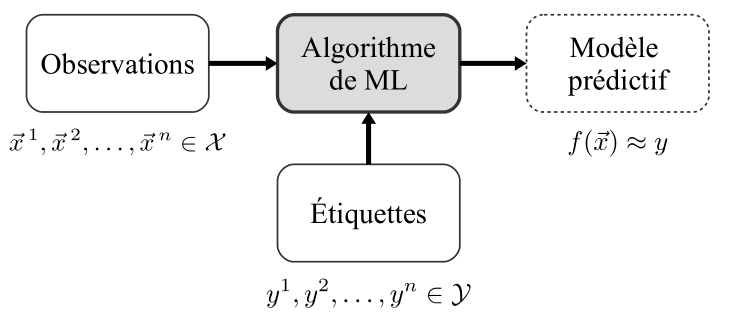
\includegraphics{fig/fig1.png}
\end{frame}

\begin{frame}
\begin{itemize}
\tightlist
\item
  \textbf{Apprentissage non supervisé}
\end{itemize}

Dans le cadre de l'apprentissage non supervisé (unsupervised learning),
les données ne sont pas étiquetées. Il s'agit alors de modéliser les
données pour mieux les comprendre. En d'autres termes, il s''agit
d'apprendre une fonction sur les données qui vérifient certaines
propriétés.

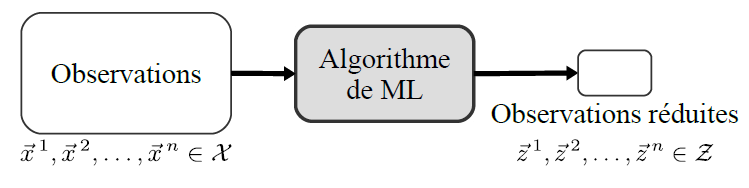
\includegraphics{fig/fig2.png}
\end{frame}

\begin{frame}
\begin{itemize}
\tightlist
\item
  \textbf{Apprentissage par renforcement}
\end{itemize}

L'apprentissage par renforcement (Deep Learning) désigne l'ensemble des
méthodes qui permettent à un agent d'apprendre à choisir quelle action
prendre, et ceci de manière autonome.

L'algorithme interagit avec son environnement en réalisant des actions
et en apprenant de ces erreurs et sucés.
\end{frame}

\hypertarget{points-clefs}{%
\section{Points clefs}\label{points-clefs}}

\begin{frame}{Points clefs}
\begin{itemize}
\item
  Un algorithme de machine learning est un algorithme qui apprend un
  modèle à partir d'exemples, par le biais d'un problème d'optimisation.
\item
  On utilise le machine learning lorsqu'il est difficile ou impossible
  de définir les instructions explicites à donner à un ordinateur pour
  résoudre un problème, mais que l'on dispose de nombreux exemples
  illustratifs.
\item
  Les algorithmes de machine learning peuvent être divisés selon la
  nature du problème qu'ils cherchent à résoudre, en apprentissage
  supervisé, non supervisé, et par renforcement.
\end{itemize}
\end{frame}

\hypertarget{logiciel-et-librairies}{%
\section{Logiciel et librairies}\label{logiciel-et-librairies}}

\begin{frame}{Logiciel et librairies}
Dans ce cours, nous utiliserons le logiciel R pour illustrer des cas
pratiques du machine learning.

Il existe plusieurs librairies (packages) pour l'implémentation du
machine learning;

caret, randomForest, e1071, mlr, nnet, rnn \ldots
\end{frame}

\end{document}
